\documentclass[11pt,titlepage]{article}

\usepackage[french,american]{babel}
\usepackage[utf8]{inputenc}
\usepackage[T1]{fontenc}
\usepackage{lmodern}
\usepackage{amsmath,amsfonts,amssymb}
\usepackage{graphicx}
\usepackage{geometry}                    % See geometry.pdf to learn the layout options. There are lots.
\geometry{letterpaper}                   % ... or a4paper or a5paper or ... 
%\geometry{landscape}                    % Activate for for rotated page geometry
%\usepackage[parfill]{parskip}           % Activate to begin paragraphs with an empty line rather than an indent
\usepackage{graphicx}
\usepackage{amssymb}
\usepackage{epstopdf}
\usepackage{color}
\usepackage[tt]{titlepic}
\usepackage{fancyhdr}
\usepackage{secdot}


% WD41, LRS/EPFL/PSI ---------------------------------------------------------
\usepackage[style=ieee, backend=bibtex]{biblatex}
\bibliography{report_2016.bib}
% Itemize under table
% from: http://tex.stackexchange.com/questions/150492/how-to-use-itemize-in-table-environment
\usepackage{booktabs}% http://ctan.org/pkg/booktabs
\newcommand{\tabitem}{~~\llap{\textbullet}~~}
\usepackage{enumitem}
\usepackage{rotating}
% ----------------------------------------------------------------------------

% Margin Setup ---------------------------------------------------------------
\topmargin=-0.45in       %
%\evensidemargin=0in     %
\oddsidemargin=-0.1in    %
\textwidth=6.8in         %
\textheight=9.0in        %
%\headsep=0.25in         %
% ----------------------------------------------------------------------------

% Titlepage ------------------------------------------------------------------
\DeclareGraphicsRule{.tif}{png}{.png}{`convert #1 `dirname #1`/`basename #1 .tif`.png}
\titlepic{
\includegraphics[width=17cm]{figures/research_plan_pic.pdf}}

\title{\textbf{Annual progress report \textcolor{blue}{2016}}}

\author{\large{\textbf{Damar Wicaksono}} \\\\
\large{\textbf{Prof. Andreas Pautz}} \\
\large{\textbf{Omar Zerkak}}\\\\\\
\Large{\textbf{Bayesian Uncertainty Quantification}} \\\\
\Large\textbf{of Physical Models} \\\\
\Large\textbf{in Thermal-Hydraulics System Code}}

\date{05.12.2016}
% ----------------------------------------------------------------------------

\begin{document}

\maketitle

% 2nd Page, an empty page ----------------------------------------------------
\pagestyle{empty}
\clearpage\mbox{}\clearpage
% ----------------------------------------------------------------------------

% Page Header, EDPY ----------------------------------------------------------
\pagestyle{fancy} \pagenumbering{arabic} \setcounter{page}{1}
\addtolength{\headheight}{\baselineskip}
\newcommand{\ffont}{\fontsize{8}{8}\selectfont}
\lhead{ECOLE DOCTORALE\\ \textit{DOCTORAL SCHOOL}}
\chead{PROGRAMME DOCTORAL EN PHYSIQUE\\ \textit{DOCTORAL PROGRAM IN PHYSICS}}
\rhead{\bfseries\ffont  
\includegraphics[width=55pt]{figures/EPFL_LOG.pdf}}
\renewcommand{\headrulewidth}{0.4pt}
% ----------------------------------------------------------------------------

% Objective of Research ------------------------------------------------------
\textcolor{white}.
\section{Objectives of research}

The  reliability of a nuclear reactor evaluation model based on codes and 
associated input (deck) is affected by the uncertainty associated with the 
codes and with the input. 
The currently adopted practice for uncertainty quantification of the 
evaluation model is done through statistical sampling where the model is 
evaluated multiple times using different values of input and code parameters 
that are represented as random variable equipped with the corresponding 
probability distribution.
Through statistical analysis of the (dispersed) output, the uncertainty 
in the predictions can be quantified.
 
In the particular case of thermal-hydraulics system codes, which can 
predict the complex dynamics of light water reactors, previous works 
have pointed out the importance of the phenomenological model parameters 
uncertainties on the codes predictions. 
System codes are valuable tools to describe complex two-phase flow 
phenomena, such as the reflooding and quenching of a pressurized water 
reactor core after a hypothetical large break loss of coolant accident.
However, such codes require the use of several parameterized physical or 
empirical models. 
However, these parameters often cannot be measured directly, might not 
have inherent physical meaning, and thus simply act as tuning parameter to
best fit specific datasets based on test facilities with various degrees of 
representativity. As such, the estimation of the uncertainty 
associated with system code parameters is mostly based on expert judgment.

The purpose of the research is to quantify the uncertainty of 
physical model parameters implemented in a thermal-hydraulics system code
(TRACE). 
The physical models of interest describe the phasic interactions in a complex 
multiphase flow during a reactor transient, namely heat, mass, and momentum 
exchanges between vapor, water and structures. 
These models are parameterized 
by physical or empirical tuning parameters, the values of which are uncertain. 
This results in uncertain code prediction of important safety quantities, such 
as the evolution of the fuel cladding temperature during a postulated reactor 
transient.
Adopting probabilistic framework to conform to the statistical uncertainty 
propagation widely practiced in the field of nuclear engineering, 
the uncertainties in the parameters are represented in form of probabilistic 
density functions or their approximation. The derivation of these functions 
is posed as an inverse statistical problem following Bayesian approach as 
the parameters themselves are not directly observable. 
In this research, a consistent methodological approach to properly pose and
solve this type of problem is to be developed and demonstrated for the 
specific phenomenon of core reflooding.
% ----------------------------------------------------------------------------

% State of Research ----------------------------------------------------------
\section{Work achieved in the past year (state of research)}

\subsection{Gaussian Process Metamodelling}

The use of meta-model (emulator, or surrogate model) representing TRACE reflood
simulation output was driven by the need to reduce computation efforts 
(CPU usage and storage) within the adopted Bayesian framework, which requires 
tens of thousands of TRACE code executions using different parameters 
values to obtain the posterior distribution with sufficient accuracy. 
The Gaussian process regression (better known as \emph{kriging} in spatial 
statistics) was adopted due to its maturity and popularity in the literature 
on applied modelling. These two properties often entail more comprehensive 
documentation, wider support, and diverse case studies.

The applicability of Gaussian process to create a meta-model for representing 
high-dimensional output (i.e., the heater rod temperature in time and 
1-dimensional space) of a FEBA TRACE model with 7 parameters has been
demonstrated in the conference article \cite{Wicaksono2016}. 
The selected 7 model parameters correspond to the 10 most important parameters
obtained from the sensitivity analysis (\cite{Wicaksono2016}) minus 3 
parameters related to the boundary conditions (inlet velocity, system 
backpressure and heater power) as only one set of experimental conditions 
was considered in the metamodel building and calibration process.
Principal component analysis (PCA) was carried out to reduce the 
high dimensionality of the output and a set of metamodels was constructed to 
approximate the principal component scores as function of the model parameters 
$\underline{\theta}$. 
That is,

\begin{equation}
	y^M(\underline{\theta};z,t) = \bar{y}^M(z,t) + \sum_{i=1}^{P_\text{tr}} v_i(z,t) \cdot w_i(\underline{\theta}) + \epsilon_\text{tr}
\end{equation}

Where $\bar{y}^M$  is the mean function, $v_i$ is the i-th principal component 
(PC or the eigenvector), $w_i$ is the $i$-th principal component score 
represented by the metamodel, and $\epsilon_\text{tr}$ is the truncation 
error. The truncation error is due to information being discarded in using fewer 
principal components ($P_\text{tr}$) than the original dimension ($P$).

The selection of the number of PC to retain $P_tr$ is usually justified by 
the amount of the explained variance carried by the selected PCs 
such as 90\%, 95\% or 99\%. 
However, in creating a Gaussian Process metamodel based on PC, the 
decision cannot be separated from the fact that PC of higher number 
tends to be harder to fit due to increasing non-linearities 
(on the contrary, the first PC tends to be the smoothest of all, 
thus easiest to fit). 
This fact is established in Figure~\ref{fig:gp_pc_conv} below that shows the 
predictivity coefficient $Q_2$ (closer to 1 is better) as function of 
training sample sizes for sequential PC calculated based on 500 independent 
validation samples obtained with the original TRACE simulation. 
From the figure it can be seen that retaining more than 
8 PCs should not significantly improve the prediction capability of 
the metamodel (note the slow and, at times, erratic convergence trends 
beyond the 4$^{\text{th}}$ PC).

\begin{figure}[h!]
	\centering
	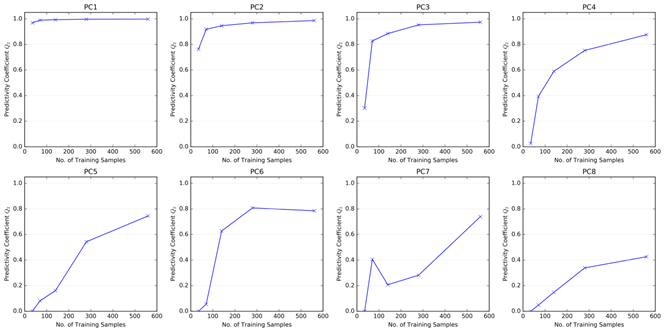
\includegraphics[scale=0.85]{figures/gp_pc_conv.png}
	\caption{The predictivity coefficient calculated using 500 
		independent TRACE validation samples as function of the 
		training size for Gaussian Process metamodels 
		with each PC scores as the output}
	\label{fig:gp_pc_conv}
\end{figure}

To check the amount of error due to retaining only a limited number of PCs to 
represent space- and time-dependent temperature output, cross-validation 
technique is used to compute the reconstruction error as function of 
increasing number of retained PCs. As can be seen in Figure~\ref{fig:rmse}, retaining only 8 PCs amounts to about, on average, 23 [K] of reconstruction 
error.

\begin{figure}[h!]
	\centering
	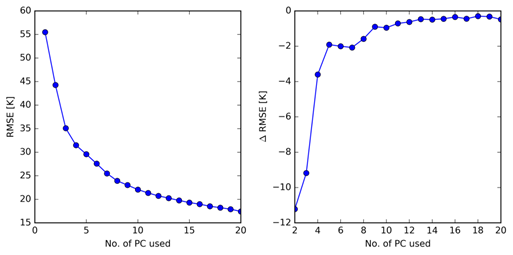
\includegraphics[scale=0.95]{figures/rmse.png}
	\caption{(\textbf{Left}) The convergence of cross-validation reconstruction
		 error (as root-mean-squared-error, RMSE of all the temperature output as function time and axial elevation) by incorporating increasing 
		 number of Principal Components (PC). (\textbf{Right}) the same 
		 measure but in terms of improvement}
	\label{fig:rmse}
\end{figure}

\subsection{Bayesian Calibration}

Also in 2016, a Bayesian calibration of selected influential TRACE reflood 
model parameters has been demonstrated in the same article 
\cite{Wicaksono2016} using only the heater 
rod temperature data from a single FEBA test (No. 216) and a normal likelihood. 
In statistical (Bayesian) formulation of computational model calibration, 
the relationship between observed data and computational model prediction is 
given by

\begin{equation}
	y^{\text{EXP}} = y^M (\underline{\hat{\theta}})+ \delta + \epsilon
\end{equation}

Where $y^\text{EXP}$ is the observed data and $y^M$  is the computational model 
prediction made at the best, but \emph{unknown}, model parameters 
($\underline{\hat{\theta}}$). 
The computational model is distorted by the 
unknown model inadequacy term $\delta$, while experimental data is 
affected by measurement error $\epsilon$.

The Bayesian approach assumes any \emph{unknown} term in a probabilistic 
sense (i.e., epistemic). 
As such, it prescribes distributional assumptions for all the unknowns 
involved in the above equation in order to formulate a likelihood function 
that can be evaluated for a given parameter value.

To formulating the posterior distribution of the model parameters, 
the present work adopted the modular Bayesian approach proposed 
by Liu \textit{et al.} (2009). 
The modular Bayesian approach is only partially Bayesian because 
at the first two steps of formulating the meta-models and the discrepancy 
term, some of the unknown hyper-parameter values are estimated separately 
and kept constant in the downstream analysis. 
As such, the uncertainties on these hyper-parameters are not taken into 
account. 
This approach is justified in many case studies by the fact that the 
hyper-parameters are often confounded with the model parameters resulting 
in non-identifiable parameters, especially if lots of model parameters 
and hyper-parameters are involved. 
With the aforementioned assumptions and using property of 
the normal distribution, the sampling data model (the likelihood) can 
be written as follows,

\begin{equation}
    y^{\text{EXP}} \sim \mathcal{N}(y^\text{M} + m_b, V \Sigma_w V^T + V_{>P_{tr}} S_{>P_{tr}} V_{>P_{tr}}^T + \Sigma_b + \sigma_\text{exp}^2 I)
    \label{eq:likelihood}
\end{equation}

Where, $V$ is a $N_{d} \times P_{tr}$ matrix given 
by $V=[v_1;v_2;\dots;v_{P_{tr}}]$ with $v_i$ is 
the $i$-th eigenvectors and  $N_d$ is the output dimension for a given 
space and time discretization, given by 
$N_d = N_{\Delta t} \times N_{\Delta z} $; 
$\Sigma_w$ is a diagonal $P_{tr} \times P_{tr}$ 
matrix with component scores prediction variance as entry;  
$S_{>P_{tr}}$ is a diagonal matrix 
with eigenvalues of higher than retained principal components;
$m_b$ and $\Sigma_b$ are the mean and the $N_d \times N_d$ covariance 
matrix of the model inadequacy (bias) term, respectively.  
$V_{>P_{tr}}$ is the equivalent matrix V for higher than retained 
principal components; 
$\sigma_\text{exp}^2$ is the variance of the experimental data; 
and $I$ is the identity matrix. 

Note that only $y^M$ and $\Sigma_w$ are functions of the model parameters.
Thus, they are to be updated during the calibration procedure. 
All the other terms (or their approximation) in Eq.~\ref{eq:likelihood} are 
obtained from experimental specifications, the preliminary PC analysis, 
the results of metamodel training, and 
the nominal values of $\underline{\theta}$, as explained in \cite{Wicaksono2016}.
This, combined with the use of metamodel to readily estimate $y^{\text{M}}(\underline{\theta})$, reduced the complexity of the problem and the 
required computational load such that an expensive Bayesian 
calibration procedure is feasible.

As for the calibration procedure itself, the posterior samples are 
generated using Markov Chain Monte Carlo 
(MCMC) method based on the likelihood function 
above and the specified prior distribution for the model parameters 
\cite{Wicaksono2016}. 
MCMC method is used to avoid difficult integration of the normalizing 
constant in the Bayes’ probability inversion theorem. 
Figure~\ref{fig:mcmc} shows the resulting histogram of the posterior samples for 
the 5-parameter model 
(the number of calibrated parameters had to be reduced from 7 to 5 due to 
identifiability issue, to be discussed in the next section).

\begin{figure}[h!]
	\centering
	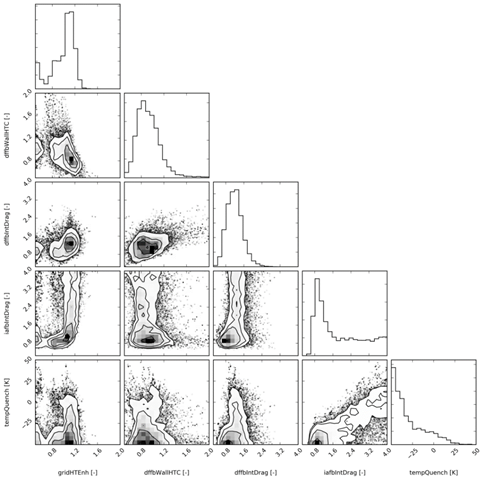
\includegraphics[scale=0.95]{figures/mcmc.png}
	\caption{Posterior of the model parameters. The 1-D marginal is shown on 
	    the diagonal while the 2-D marginal for each pairs are shown on the 
	    off-diagonal part of the plot. The contour lines on the 2-D marginal
	    plots correspond to 1-, 2-, and 3-$\sigma$ levels}
	\label{fig:mcmc}
\end{figure}

The results of calibrating the 5-parameter model are presented in corner 
plot in Figure~\ref{fig:mcmc}. 
A corner plot depicts all the one-dimensional 
and, in pairwise, the two-dimensional marginals of the posterior samples. 
It provides information on possible correlation between parameters. 
As can be seen, the most constrained parameters are the 
\textbf{dffbWallHTC}\footnote{The wall heat transfer coefficient in the post-CHF dispersed flow regime (DFFB)}  
and the \textbf{dffbIntDrag}\footnote{The interfacial drag coefficient in the post-CHF DFFB regime}, 
while the \textbf{iafbIntDrag}\footnote{The interfacial drag coefficient in the post-CHF inverted annular film boiling regime} 
is the least constrained (see upper half values of the range).
This result is supported by the analysis in \cite{Wicaksono2016a}, 
which found the temperature output to have a much smaller sensitivity to 
\textbf{iafbIntDrag} than to the two previous parameters. 
The calibration of \textbf{gridHTEnh}\footnote{Spacer grid heat transfer enhancement coefficient} 
is also peculiar as if the lower bound of its variation range was less 
constrained.
In \cite{Wicaksono2016} it was indeed found that only upper half values of 
the parameter range were influential to the temperature output. 
Finally, the quench temperature calibration result indicates the need for a 
negative shift of parameter \textbf{tempQuench}\footnote{Quench temperature} 
for higher consistency with data and the error model used. 
As for this unanticipated shift, one should recall that only one test 
has been considered here (No. 216) thus a risk of over-fitting, 
but also that FEBA data are not part of the official validation database of 
the TRACE code for reflooding. 

To validate the posterior distribution of model parameters obtained from the 
calibration using FEBA Test No. 216, uncertainty propagation for temperature 
prediction of FEBA Test No. 214 has been obtained and is shown in 
Figure~\ref{fig:uqrun}. 
As can be seen the posterior parameters distributions yield narrower 
uncertainty for the temperature prediction, thus confirming the potential 
of the developed calibration method.

\begin{figure}[h!]
	\centering
	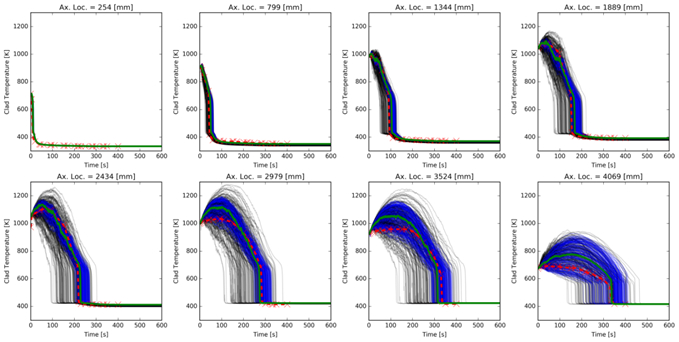
\includegraphics[scale=0.95]{figures/uqrun.png}
	\caption{Posterior temperature prediction of FEBA Test No. 214 (blue lines)
	    obtained by propagating the posterior distribution of model parameters
	    obtained from FEBA Test No. 216. The prior temperature predictions are 
	    shown in black in the background. The nominal prediction and 
	    experimental data are shown in green and red dashed lines, respectively.}
	\label{fig:uqrun}
\end{figure}

% ----------------------------------------------------------------------------

% Current State of Work ------------------------------------------------------
\section{Current state of work}

Initially, the calibration process was carried out on the full 7-parameter 
model using FEBA heater rod temperature evolution data at 8 different axial 
locations. 
It was found that the Markov Chain failed to converge as indicated by the 
lack of mixing shown in Figure~\ref{fig:nonconv}. 
The trace or sequence of posterior samples during the MCMC iterations can 
provide indication on the convergence of the chain, thus reliability of the 
results. As can be seen, the algorithm failed to concentrate the posterior 
on a specific range of values. 
Instead, the whole range of the prior values seems to be plausible.

\begin{figure}[h!]
	\centering
	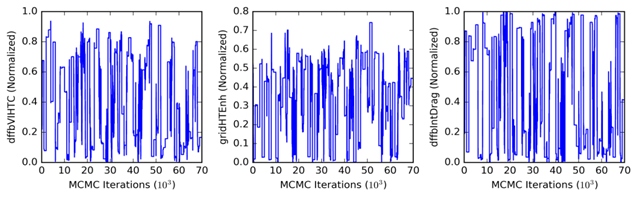
\includegraphics[scale=0.90]{figures/nonconv.png}
	\caption{Trace plots of three selected parameters values during 
	    MCMC iterations showing no convergence of the 7-parameter
	    model calibration}
	\label{fig:nonconv}
\end{figure}

Diagnosis on the problem revealed collinearity between two pairs of 
parameters: \textbf{dffbVIHTC}-\textbf{dffbIntDrag} and 
\textbf{iafbWallHTC}-\textbf{iafbIntDrag}. 
For each flow regime, namely DFFB and IAFB, 
the effect on the output of changes in one parameter 
related to heat transfer can be compensated in the same manner 
by changes in the other parameter related to interfacial drag, due to 
collinearity. 
During the calibration, this compensation effect resulted in wide range of 
collinear parameter values that cannot be constrained by the rod temperatures 
data alone. 
Figure~\ref{fig:collinear} illustrates the problem of collinearity between the 
\textbf{dffbVIHTC}-\textbf{dffbIntDrag} pair. 
In \cite{Wicaksono2016}, the issue was side-stepped by excluding the less 
influential parameter in each pair from the calibration process.

\begin{figure}[h!]
	\centering
	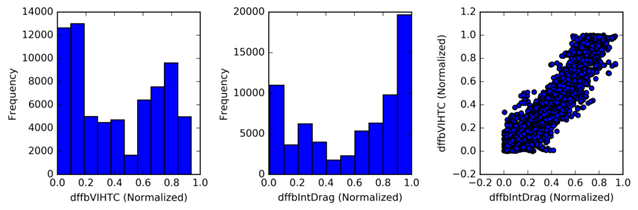
\includegraphics[scale=0.90]{figures/collinear.png}
	\caption{Non-converging distributions of two collinear parameters
	    \textbf{dffbVIHTC} and \textbf{dffbIntDrag}}
	\label{fig:collinear}
\end{figure}

The issue of model identifiability was not well explored in the nuclear 
engineering and safety community, judging from the zero relevant results 
in the recent publications of \textit{Nuclear Science and Engineering}, 
\textit{Nuclear Technology}, \textit{Nuclear Engineering and Design}, 
\textit{Progress in Nuclear Energy}, and \textit{Annals of Nuclear Energy}. 
However, the issue was often raised in chemical engineering, 
environmental science, and system biology modelling although consensus 
on the resolution of the issue is yet to be found. 
In principle, the proposed solutions to the model identifiability problem 
can be divided into two broad categories:

\begin{enumerate}
    \item Using the result of sensitivity analysis to select a subset of model 
    parameters that are systematically identifiable using calibiration data 
    at hand. 
    Such an approach was already adopted though with less rigor in 
    \cite{Wicaksono2016} where only a subset of the 
    initial set of influential model parameters was eventually retained 
    for calibration.
    One of the difficulty in such approach is to find a parameter that preserves
    the physical meaning of both collinear parameters.
    This is not always possible, as it was the case for the problem at hand.
    
    \item Using additional model response – experimental data pair to break the 
    collinearity. 
    In essence, the calibration problem will become a 
    multi-objective optimization problem, seeking to obtain plausible parameters 
    values that are in accordance to the competing objectives. 
    Depending on several factors such as the inherent correlation between 
    different types of measurements and/or code outputs, the identifiability 
    of the parameters cannot be guaranteed and the actual implementation of the 
    approach remains an open issue. 
\end{enumerate}

The identifiability issue will be investigated  in the particular case of reflooding by incorporating additional source of information (e.g., measured axial pressure drops and/or liquid carry-over) and thus make good use of the FEBA data at hand. If successful, the approach will provide additional relevant novelty to the doctoral research.

% ----------------------------------------------------------------------------

% Calendar -------------------------------------------------------------------
\section{Calendar of upcoming work}

The proposed upcoming works and the timeframe were detailed in the separate 
document which was submitted to the EPFL Doctoral School of Physics to 
justify an extension of the doctoral research duration \cite{Wicaksono2016d}.
Table~\ref{tab:proposedworks} summarizes the proposed works, while Figure~\ref{fig:gantt} gives their respective time frame.

\begin{table}[h!]
	\caption{Summary of the Proposed Works
	}
	\label{tab:proposedworks}
	\begin{center}
		\footnotesize
		\begin{tabular}{p{3cm} l p{2.5cm} l}
% Header ----------------------------------------------------------------------
			\toprule[1.5pt]
			Objectives
			& Tasks 
			& Expected Efforts 
			& Publication Plan \\ \hline \\
% 1st Element -----------------------------------------------------------------
			Metamodel Building and Validation
			& \parbox[c]{0.3\textwidth}{%
				Investigate the effect on the metamodel construction of using
				different design for training, covariance function, diagnostic
				measure, and validation schemes.             %Task Description
			} 
			& \parbox[c]{0.2\textwidth}{
		        1 Month} 
			& \parbox[c]{0.3\textwidth}{%
				A technical report on important aspects of the building and application of GP metamodel} \\ \\ \hline
% 2nd Element -----------------------------------------------------------------
				\parbox[c]{0.18\textwidth}{Bayesian calibration incorporating data from different ex\-perimental conditions} 
				& \parbox[c]{0.3\textwidth}{%
					\begin{itemize}[leftmargin=1em,itemsep=1pt,parsep=0pt]\raggedright%
						\item Review previous works on taking into account and different physical condition into calibration results
						\item Conduct Bayesian calibration on the basis of temperature data from all the FEBA Series 1 tests
					\end{itemize}}  
				& \parbox[c]{0.2\textwidth}{%
					2 Months
					}
				& \parbox[c]{0.3\textwidth}{%
					\begin{itemize}[leftmargin=1em,itemsep=1pt,parsep=0pt]\raggedright%
						\item A journal article on extension of Bayesian 
						calibration of TRACE reflood model to all 6 FEBA 
						Series I tests temperature data
						\item A short technical description report on the
						application of Bayesian approach for model calibration
					\end{itemize}} \\ \hline
% 3rd Element -----------------------------------------------------------------
				\parbox[c]{0.18\textwidth}{Bayesian calibration incorporating additional code re\-sponses \- experimental data pair to tackle identifiability issue}
				& \parbox[c]{0.3\textwidth}{
					\begin{itemize}[leftmargin=1em,itemsep=1pt,parsep=0pt]\raggedright%
						\item Conduct global sensitivity analysis for TRACE model of FEBA for other responses
						\item Construct Gaussian process metamodel for additional model responses
						\item Investigate ways to incorporate additional model response(s) in the calibration process
					\end{itemize}}
				& \parbox[c]{0.2\textwidth}{%
					3 Months
					}
				& \parbox[c]{0.3\textwidth}{
					A journal article on the use of additional system response of FEBA TRACE model to tackle identifiability issue} \\	\hline
% 4th Element -----------------------------------------------------------------
				\parbox[c]{0.18\textwidth}{Method Validation: Uncertainty propagation in ACHILLES reflood experiment}
				& \parbox[c]{0.3\textwidth}{
					\begin{itemize}[leftmargin=1em,itemsep=1pt,parsep=0pt]\raggedright%
						\item Extraction of experimental data
						\item Review of previously developed TRACE models for selected ACHILLES Tests
						\item Global sensitivity analysis of the TRACE models
						\item Propagation of model parameter uncertainty
					\end{itemize}}
				& \parbox[c]{0.2\textwidth}{%
					3 Months} 
				& \parbox[c]{0.3\textwidth}{%
					A journal article draft on the independent validation of the
					proposed methodology against ACHILLES data}\\
% End ------------------------------------------------------------------------
			\bottomrule[1.5pt]
		\end{tabular}
	\end{center}
\end{table}
% ----------------------------------------------------------------------------

\begin{sidewaysfigure}[ht]
	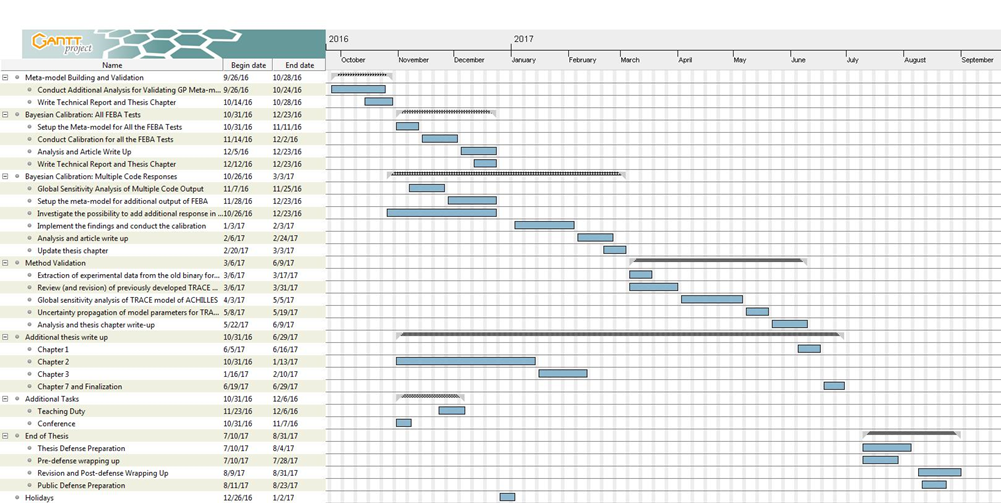
\includegraphics[scale=0.85]{figures/gantt.png}
	\caption{Calendar of upcoming works}
	\label{fig:gantt}
\end{sidewaysfigure}


\section{Other activities (teaching duties, etc.) and remarks}

\subsection{Nuclear Computations Lab (ETH-531)}

A teaching activity was carried out for a part of the Nuclear Computations Lab 
course organized at PSI (one chapter, entitled ``Basic Thermal-hydraulics'', out of 
6 chapters in total). 
The course is part of the EPFL/ETHZ Nuclear Engineering Master Program and has 
now become an obligatory course for students.
A full day was dedicated for a lecture session followed by a hands-on computer
simulation session using the TRACE code.
Ten students participated in the course this semester, all of whom showed good 
enthusiasm.

\subsection{Completion of the OECD/NEA PREMIUM Benchmark}

In 2016, written contributions and reviews were made in relation to the finalization and the release of two OECD/NEA international reports 
on PREMIUM (\cite{Reventos2016, Sanz2016}). 
More details can be found in \cite{Wicaksono2016b}, 
which summarizes the PSI contribution to PREMIUM 
and includes a discussion on the lessons learned from this benchmark.


\section{Scientific publications, conference contributions, \& presentations}

\nocite{Wicaksono2016}
\nocite{Wicaksono2016a}
\nocite{Wicaksono2016b}
\nocite{Wicaksono2016c}
\nocite{WicaksonoPPTa}
\nocite{WicaksonoPPTb}
\nocite{WicaksonoPPTc}

\printbibliography[heading=none]
\clearpage

% Signature Page -------------------------------------------------------------
\newpage
\textcolor{white}.\\\\
\noindent \textbf{Comments by the thesis advisor(s)}\\\\
\noindent\textbf{Prof. A Pautz}\\\\
............................................................................
............................................................................\\\
............................................................................
............................................................................\\\
............................................................................
............................................................................\\\
............................................................................
............................................................................\\\
............................................................................
............................................................................\\\
............................................................................
............................................................................\\\
............................................................................
............................................................................\\\\\
%
\noindent\textbf{O. Zerkak}\\\\
............................................................................
............................................................................\\\
............................................................................
............................................................................\\\
............................................................................
............................................................................\\\
............................................................................
............................................................................\\\
............................................................................
............................................................................\\\
............................................................................
............................................................................\\\
............................................................................
............................................................................\\\

\section*{\underline{Signatures}\\}
\noindent \textbf{Thesis advisor}\hspace{6.25cm}..............................................................................\vspace{0.5cm}\\

\noindent \textbf{Thesis co-advisor}\hspace{5.7cm}..............................................................................\\
\noindent  (if applicable)\\\\

\noindent \textbf{With his signature, the candidate confirms that he took note of the above comments.}\\\\
\textbf{Candidate}\hspace{7cm}..............................................................................\vspace{0.5cm}\\

\noindent \textbf{Date}\hspace{8.05cm}..............................................................................\\

\vspace{0.8cm}
\begin{center}
%\textbf{Up to 5 pages in total}
\end{center}
\begin{center}
\textbf{To be returned to:} \textcolor{green}{EPFL-EDPY / Station 3 / 1015 Lausanne / Suisse}
\end{center}
% ----------------------------------------------------------------------------
\end{document}  